\chapter{Troubleshooting}
\label{troubleshooting}

Troubleshooting can be frustrating when you are tired. You need plenty
of gumption and an open mind. Difficult problems are usually a
combination of two or more problems. So \textbf{do not attempt if you
are tired or in a hurry} .

\section{Oscilloscope}
\label{oscilloscope}

The best tool for debugging an embedded system is an oscilloscope.

\begin{enumerate}
\item
  Use x10 probes.
\item
  Use the correct probes for the scope so that they can be automatically
  detected.
\item
  Compensate the probes by clipping to the probe test signal on the
  scope and adjusting the variable capacitor in the probe to ensure a
  square wave without undershoot or overshoot. This is one of the few
  times you are allowed to use the autoscale button!
\end{enumerate}

\subsection{Normal mode}
\label{normal-mode}

This mode is for measuring transient or non-repetitive signals. It will
only refresh the display if a trigger event is detected.

It is useful to increase the \emph{trigger holdoff} to prevent
triggering on multiple edges of a waveform. By default, it is set to a
ridiculously small value.

\subsection{Auto mode}
\label{auto-mode}

This mode is for measuring AC or DC signals. It is like normal mode but
if it does not detect a trigger it will automatically refresh the
display.

\section{SAM4S not detected by OpenOCD}
\label{sam4s-not-detected-by-openocd}

If a program has not been loaded:

\begin{enumerate}
\item
  Check orientation of the SAM4S.
\item
  Check soldering of the SAM4S pins under a microscope. Giving
  each pin a push with a sharp spike can reveal a poorly soldered joint.
\item
  Check 3.3 V and 1.2 V power rails.
\item
  Check the serial wire debug (SWD) signals, see
  \protect\hyperref[debugging]{Debugging serial wire debug (SWD)}.
\end{enumerate}

If a program has been loaded:

\begin{enumerate}
\item
  Check the crystal oscillator, see
  \protect\hyperref[checking-the-crystal-oscillator]{Checking the
  crystal oscillator}.
\item
  Erase the flash memory by connecting the ERASE pin to 3.3 V, re-enable
  booting from flash, and reprogram the SAM4S with an LED flash
  program.
\end{enumerate}

\subsubsection{Debugging serial wire debug (SWD)}
\label{debugging-serial-wire-debug-swd}

\program{OpenOCD} periodically polls to see if the SAM4S is alive.
These occur every 100\,ms.

\begin{figure}
\centering
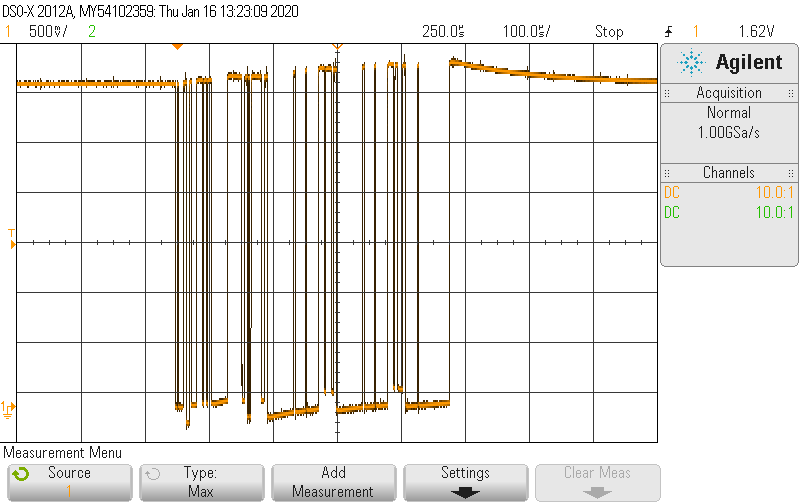
\includegraphics[height=2.60417in]{figs/OpenOCDPollingGood.png}
\caption{OpenOCD periodic poll when it gets a response from the SAM4S.}
\end{figure}

\begin{figure}
\centering
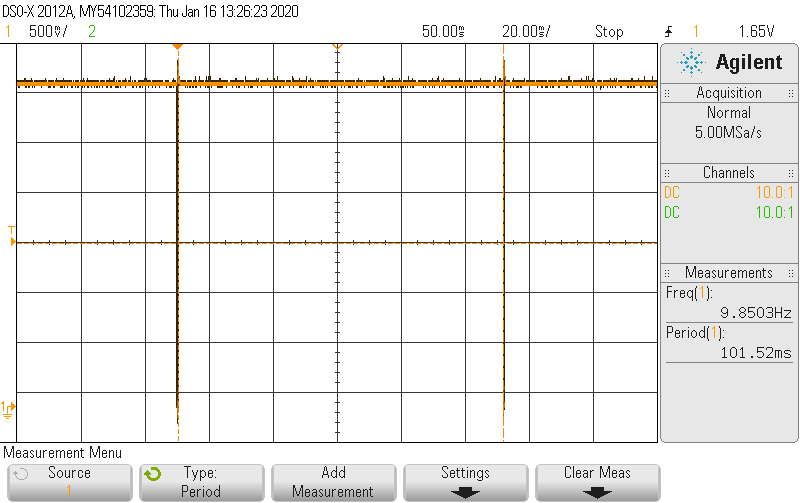
\includegraphics[height=2.60417in]{figs/OpenOCDTimingGood.png}
\caption{OpenOCD polls every 100\,ms while connected.}
\end{figure}

OpenOCD polls less often when it does not get a response. The period
increases to 6300\,ms.

\subsection{Checking the crystal oscillator}
\label{checking-the-crystal-oscillator}

When the SAM4S is first powered up it uses an internal oscillator.
However, when a program is loaded it switches to the main oscillator
that uses the external crystal. If there is a problem with the crystal
oscillator the SAM4S will not run since it has no clock. Moreover,
\program{OpenOCD} will then fail to communicate with the SAM4S.

\begin{figure}
\centering
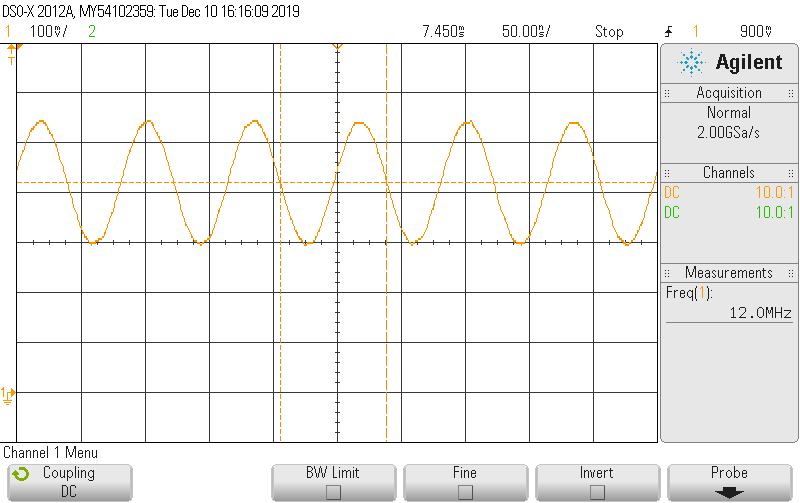
\includegraphics[height=2.60417in]{figs/ClockSignal.png}
\caption{12\,MHz clock sine wave.}
\end{figure}

\mtodo{Add scope picture of CPU clock signals when not working}

\begin{enumerate}
\item
  Connect a scope pin to the XOUT pin. A 12\,MHz sinewave should be
  visible.
\item
  If there is no sinewave:

  \begin{enumerate}
  \item
    Measure the voltage on the VDDPLL pin of the MCU with a scope. This
    should be 1.2 V to power the oscillator.
  \item
    Check the bypass capacitors across the crystal. These should be
    approx. 20 pF.
  \end{enumerate}
\end{enumerate}

\subsection{Checking the clock}
\label{checking-the-clock}

The SAM4s has multiple clock sources:

\begin{enumerate}
\item
  Internal fast RC oscillator (this is selected when the SAM4S is first
  ever used).
\item
  Internal slow RC oscillator (this can be selected to save power).
\item
  Main oscillator using external crystal.
\end{enumerate}

The SAM4S uses a phase-locked-loop (PLL) to multiply the frequency of
the clock source to provide the CPU clock. Sometimes the PLL will run
without a clock source and thus will generate an unexpected frequency.

The clock frequency can be checked by connecting a scope to a peripheral
pin that generates a clock, e.g., PWM, SCK, TXD.

\section{USB serial}
\label{debugging-usb}

USB is a complicated protocol and there are many possibilities why it
does not work.

  \begin{itemize}
  \item
    Check that the termination resistors are 27\,ohms.
    
  \item Check the SAM4S is running at the correct frequency of
    96\,MHz. Check the SAM4S XIN pin with an oscilloscope for a
    12\,MHz sinusoid. Note, the oscillator is not enabled unless a
    program has been loaded and running. If a 12\,MHz signal is not
    found, check the MCU solder connections under a microscope. Also
    check that the VDDPLL pin has 3.3\,V.
  \end{itemize}

  If the USB serial connection drops characters:
  %
 \begin{itemize}
 \item Add a delay before sending data.  This is because the driver
   takes a while to set up the connection after the USB cable is
   plugged in If you try to send some data in this time, the data gets
   stored into a ring buffer for later transmission.  However, the
   ring buffer is not large and once it is filled, the USB serial
   driver will drop characters.
 \end{itemize}

\section{Testing peripherals}
\label{testing-peripherals}

 
\subsection{Motors}
 
\subsection{Debugging PWM}
\label{debugging-pwm}

If PWM does not work:

\begin{enumerate}
\item
  Check the SAM4S pin since not every pin can be a PWM signal
\item
  Check the definition in the configuration file \file{target.h}
\end{enumerate}

If the PWM frequency is wrong:

\begin{enumerate}
\item
  Check the clock frequency, see \hyperref[checking-the-clock]{Checking the clock}.
\item
  Check your program.
\end{enumerate}

If the PWM duty is wrong:

\begin{enumerate}
\item
  Check your program. The duty is specified as an integer in parts per
  thousand. (e.g. 1000 = 100\% duty cycle; 50 = 5\% duty cycle)
\end{enumerate}

\begin{figure}
\centering
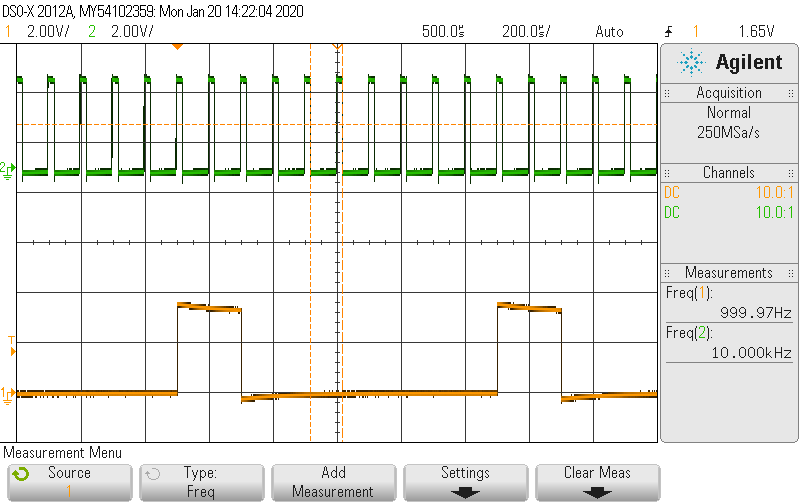
\includegraphics[height=2.60417in]{figs/PWM_2.png}
\caption{Two PWM signals at 1\,kHz and 10\,kHz.}
\end{figure}


\subsubsection{Testing the H-bridge}
\label{testing-the-h-bridge}

\begin{enumerate}
\item The \sig{nFAULT} pin should be high.  Note, this is an
  open-drain pin and requires a pullup resistor to 3V3 to make it
  work.  Without this resistor, this pin will always read low, fault
  or no fault.

\item The \sig{nSLEEP} pin needs to be high to enable the chip.

\item Check that the capacitor connected to the \sig{INT} pin is
  2.2\,$\mu$F and not 2.2\,nF.
\end{enumerate}


\subsection{IMU}
\label{imu}

\subsection{Debugging I2C}
\label{debugging-i2c}

\begin{enumerate}
\item
  I2C/TWI requires external pull-up resistors for the clock (TCK) and
  data (TDA) signals.
\item
  TWI channel 1 (TWI1) uses \pin{PB4} and \pin{PB5}. However, these are configured
  on boot as JTAG pins. You can disable this, see
  \hyperref[disabling-jtag-pins]{disabling JTAG pins}.
\end{enumerate}

\mtodo{Add scope picture of I2C signals}

\mtodo{Add scope picture of I2C signals with no acknowledge}

\subsection{NRF24L01+ radio}
\label{nrf24l01-radio}

For the radio to work you need:

\begin{enumerate}
\item
  A working SPI interface.
\item
  The correct channel and address.
\item
  A well filtered power supply for the radio.
\item
  A channel with little interference (note, some channels are shared
  with WiFi and Bluetooth and may be less reliable).
\end{enumerate}

If nothing works, check:

\begin{enumerate}
\item
  For transmission the CE pin should be low; for reception the CE pin
  should be high.
\item
  Check that the SPI clock SCK, MOSI, and MISO signals are driven when
  the radio is configured (note, the MISO signal is tristate when CS is
  high).
\item
  Check that the SPI CS signal is driven low for each transmitted byte.
\end{enumerate}

If the radio transmits but not receives, check:

\begin{enumerate}
\item
  The IRQ pin is driven low (this indicates that a packet has been
  received).
\item
  The power supply. The radio requires a well filtered power supply
  otherwise the range will be limited on reception. Preferably, the
  device should have its own 3V3 regulator with a low-pass RC filter
  comprised of a series resistor and large capacitor (say 22\,$\mu$F) or a
  low-pass LC filter made with a ferrite bead and capacitor.
\end{enumerate}

\textbf{Note}, by default the radio waits for an auto-acknowledgement
from the receiver device. This acknowledgement is performed in hardware.
If no acknowledgement is received, it retries for up to 15 times. The
auto-acknowledgement and number of retries can be configured in
software.

\subsubsection{Checking the radio power supply}
\label{checking-the-radio-power-supply}

\mtodo{Add scope picture of expected radio power supply voltage}

\subsubsection{Debugging SPI}
\label{debugging-spi}

Check:
%
\begin{enumerate}
\item The device chip select signal is driven low.
\item The \pin{SCK} signal toggles while the chip select is low.
\item The \pin{MOSI} signal does something while the chip select is low.
\end{enumerate}
%
The \pin{MISO} signal is usually tri-state and is driven by the
device when the chip select is low.

The SPI standard is rather loose and there are four modes to confuse
the unwary; these are due to two clock polarity modes and two clock
phase modes.  When using the wrong mode, the read data can be
bit-shifted or unreliable.

\mtodo{Add scope picture of SPI signals}

\section{Other problems}
\label{faq}

\begin{itemize}
\item
  \emph{\program{OpenOCD} does not run}. The most common problem is that the
  USB permissions are not correct.
\item
  \emph{A program does not correctly build after a file has been
  changed}. Every now and then the file timestamps are incorrect (this
  is a common problem with network drives due to a skew in the clocks)
  and make will not correctly rebuild a file. Running \textbf{make
  clean} will remove the existing dependency and object files so you can
  start afresh.
\item
  \emph{A program hangs.} This can be observed by an LED no longer
  flashing. There are a number of reasons:

  \begin{itemize}
  \item
    The program is stuck in an infinite loop. Note, an embedded system
    should only have an infinite loop for the main loop; all other loops
    should have a timeout condition.
  \item
    The program has crashed trying to access invalid memory. Usually
    this is due to buffer overflow or dereferencing uninitialised
    pointers (say by not calling \code{radio_init}). Try running
    'make debug'. This will start the
    \protect\hyperref[debugging]{debugger} and attach to your MCU. If
    the debugger says that your program has stopped in
    '\_hardfault\_handler', then your program is likely to have accessed
    invalid memory. Use the 'bt' command to print a stack trace to see
    how your program went astray.
  \end{itemize}
\item
  \emph{The output of the 3V3 regulator works fine when powered from USB
  but gives 6 V when powered from a 7.2 V battery}. Check that the 7.2 V
  is not connected directly to a SAM4S pin (say for battery monitoring)
  since this will cause an ESD protection diode inside the SAM4S to
  conduct.
\end{itemize}

